\linespread{1.13}\selectfont

%%%%%%%%%%%%%%%%%%%%%%%%%%%%%%%%%%%%%%%%%%%%%%%%%%%%%%%%%%%%%%%%%%
%%%%%%%%%%%%%%%%%%%%%%%%%%%%%%%%%%%%%%%%%%%%%%%%%%%%%%%%%%%%%%%%%%
\chapter{Создание сервиса прогнозирования}
%%%%%%%%%%%%%%%%%%%%%%%%%%%%%%%%%%%%%%%%%%%%%%%%%%%%%%%%%%%%%%%%%%
%%%%%%%%%%%%%%%%%%%%%%%%%%%%%%%%%%%%%%%%%%%%%%%%%%%%%%%%%%%%%%%%%%
\section{Подготовка инструментов}
Необходимо установить IDE NetBeans, при установке указать что требуется установить сервер приложений GlassFish. Его можно заменить на аналоги, например Wildfly.  

Для начала необходимо создать новый java проект в IDE, и указать что он будет web приложением. Создание такого типа приложения позволит строить распределенную систему из отдельных компонент без привязки к физическому расположению. 

\begin{figure}[h!]
\center
	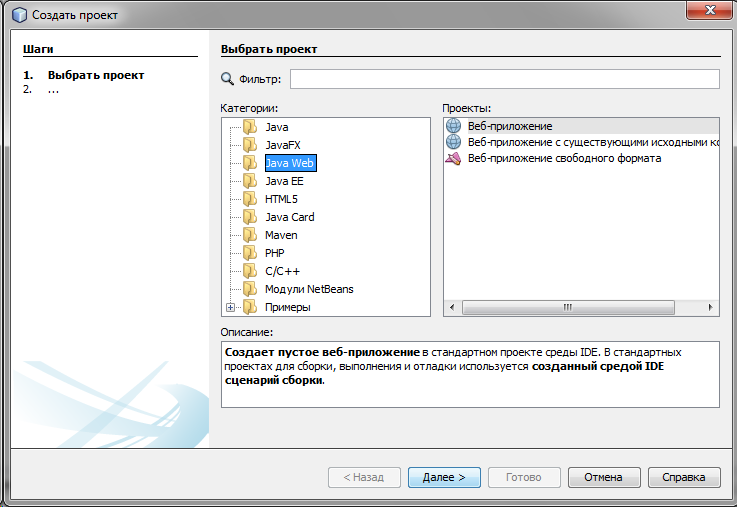
\includegraphics[scale=0.8]{service/1.png}
	\caption{Тип проекта}
	\label{pict:projecttype}
\end{figure}

Задаем наименование проекта, указываем его расположение. Проект, созданный по данной инструкции будет использовать ant в качестве системы управления сборкой. 

\begin{figure}[h!]
\center
	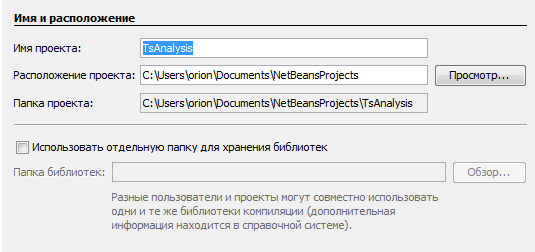
\includegraphics[scale=0.8]{service/2.png}
	\caption{Название проекта}
	\label{pict:projectname}
\end{figure}

Далее нужно указать IDE, на какой сервер будет разворачиваться приложение. Эта настройка позволят запускать приложение напрямую из IDE. Разумеется, если приложение впоследствии будет, развернуто на другом сервере то настройки указанные здесь никак не помешают этому.

\begin{figure}[h!]
\center
	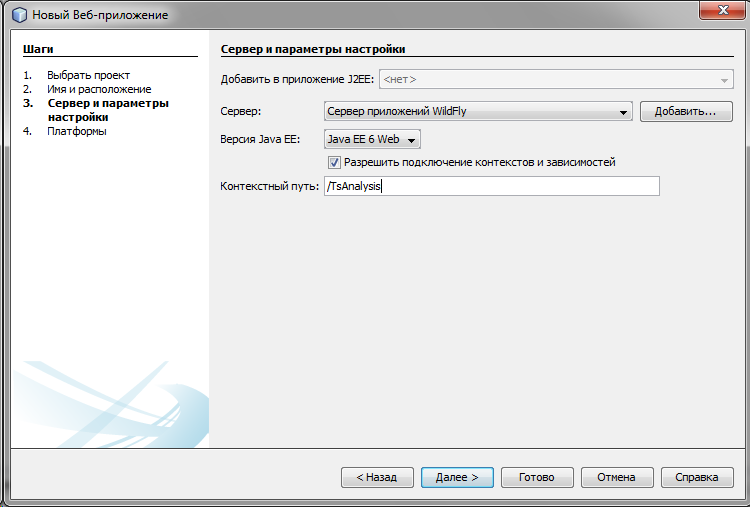
\includegraphics[scale=0.8]{service/3.png}
	\caption{Выбор сервера}
	\label{pict:projectserver}
\end{figure}
